\documentclass[twoside, 10pt]{article}

\usepackage{geometry}
\geometry{outer=3em, inner=2.2cm, top=6em, bottom=4em, headheight=\paperheight}
\usepackage[export]{adjustbox}
\usepackage{array}
\usepackage{amsmath}
\usepackage{amsfonts}
\usepackage{fancyhdr}
\pagestyle{fancy}
\fancyhf{}
\lhead{Algebra II - BASE}
\chead{Function Compositions}
\rhead{AO Make, Page \thepage}
\usepackage{lastpage}
\usepackage{xcolor}
\usepackage{enumitem}
\usepackage{pifont}
\usepackage{graphicx}
\graphicspath{{../img}}
\usepackage{pgfplots}
\pgfplotsset{compat=1.18}
\usepackage{tabularx}
\usepackage{tikz}
\usetikzlibrary{patterns}

\newcommand{\R}{\mathbb R}
\newcommand{\e}{{\rm e}}
\newcommand{\pobr}[1]{\left\langle#1\right\rangle}
\newcommand{\norm}[1]{\lVert #1 \rVert}
\newcommand{\abs}[1]{\lvert #1 \rvert}

\DeclareMathOperator{\xd}{d\!}
\DeclareMathOperator{\proj}{proj}

\title{}
\date{}

\begin{document}
\noindent
{\large
First Name \rule{6em}{.1pt}\hspace{\stretch{1}}Last Name \rule{6em}{.1pt}\hspace{\stretch{1}} Due \rule{1.5em}{.1pt} -- \rule{1.5em}{.1pt} -- \rule{1.5em}{.1pt}\hspace{\stretch{1}} Period \rule{2em}{.1pt}\hspace{\stretch{1}} Score \rule{2em}{.1pt}
}
\vspace{1em}

\begingroup
\renewcommand{\arraystretch}{1.5}
\begin{center}
\tiny
{
\begin{tabularx}{\textwidth}{|X|X|X|X|X|X|}
\hline
\bf BE PRECISE & \centerline{Integrating} & \centerline{Applying} & \centerline{Practicing} & \centerline{Acquiring} & \centerline{Awaiting Evidence} \\
\hline
I can calculate accurately and efficiently, and be precise in all of my math.&
Selects and applies the correct procedure and solves all routine AND integrating problems.

AND

Expresses the answer to the correct level of precision needed for the problem (including the correct rounding, units, math symbols, labeling, graphing, vocab…)
&Selects and applies the correct procedure and solves all routine problems.


AND

Expresses the answer to the correct level of precision needed for the problem (including the correct rounding, units, math symbols, labeling, graphing, vocab…)
&Selects and applies the correct procedure and solves most routine problems.


AND

Expresses the answer to the correct level of precision needed for the problem (including the correct rounding, units, math symbols, labeling, graphing, vocab…)
&Selects and applies the correct procedure and solves some routine problems.


AND

Attempts to express the answer to the correct level of precision needed for the problem (including the correct rounding, units, math symbols, labeling, graphing, vocab…).
&Selects and attempts to apply the correct procedure for some routine problems.\\
\hline
\bf Criteria&\multicolumn{5}{l|}{\parbox[c][4em]{.8\textwidth}{}}\\
\hline
\end{tabularx}
}
\end{center}
\endgroup

\begin{enumerate}
\item Create a problem of composing two polynomial functions.
\\[2em]
Let $f(x)=\rule{15em}{.1pt}$ and $g(x) = \rule{15em}{.1pt}$. 
\begin{enumerate}
\item
({\bf Instruction}: Fill the blank with a number.)
Find $f(g(\rule{2em}{.1pt}))$.
\vspace{\stretch{1}}
\item
({\bf Instruction}: Fill the blank with a first degree polynomial.)
Find $g(\rule{5em}{.1pt})$ and simplify.
\vspace{\stretch{1}}
\item
Find $(g\circ f)(x)$ and simplify.
\vspace{\stretch{1}}
\end{enumerate}
\clearpage

\item
Create a problem of composing two functions via tables.

({\bf Instruction:} Define your functions by completing the tables.)

\begingroup
\renewcommand{\arraystretch}{2}
\begin{tabular}{cc}
\begin{tabularx}{0.45\textwidth}{|>{\centering}X|X|X|X|X|X|X|}
\hline
x&&&&&&\\
\hline
f(x)&&&&&&\\
\hline
\end{tabularx}\hspace{\fill}
&
\begin{tabularx}{0.45\textwidth}{|>{\centering}X|X|X|X|X|X|X|}
\hline
x&&&&&&\\
\hline
g(x)&&&&&&\\
\hline
\end{tabularx}
\end{tabular}
\endgroup

({\bf Instruction}: Fill each blank with a number.)
Find the following using the tables above:
\begin{enumerate}
\item
$(g\circ f)(\rule{2em}{.1pt})$
\vspace{\stretch{1}}
\item
$(f\circ g)(\rule{2em}{.1pt})$
\vspace{\stretch{1}}
\end{enumerate}

\item
Create a problem of composing two functions via graphs.

({\bf Instruction}: Make the graphs of your functions below. Label them clearly.)

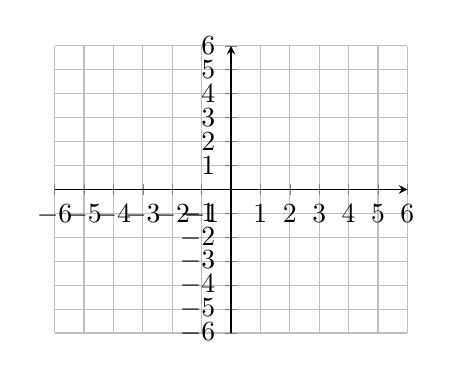
\begin{tikzpicture}[baseline=(current bounding box).middle]
\begin{axis}[
axis lines=middle,
grid=both,
xtick distance=1,
ytick distance =1,
ymin=-6, ymax=6,
xmin=-6, xmax=6,
width = 0.5\textwidth
]
\end{axis}
\end{tikzpicture}

The graph above contains the lines for $h(x)$ and $k(x)$. Use it to find the following $(h\circ k)(\rule{3em}{.1pt})$. ({\bf Instruction}: Fill the blank with a number.)
\vspace{\stretch{1}}
\end{enumerate}

\end{document}